\documentclass[11pt]{article}
\usepackage{graphicx}
\usepackage{amssymb}
\usepackage{color}

\pagestyle{empty}

\textwidth = 6.5 in
\textheight = 9 in
\oddsidemargin = 0.0 in
\evensidemargin = 0.0 in
\topmargin = 0.0 in
\headheight = 0.0 in
\headsep = 0.0 in
\parskip = 0.2in
\parindent = 0.0in


\begin{document}
{\large {\bf CMPT 202 - Merge Sort}} 

1. The {\bf Merge Sort} has two phases: (1) a {\it splitting} phase, followed by a (2) {\it merge} phase. The splitting phase works by splitting $N$ numbers from one list into $N$ lists each containing 1 number. Complete the splitting phase for the following numbers:

\begin{figure}[h]
\centerline {
\includegraphics[width=3in]{ms-1.png}
}
%\caption{Example binary tree {\tt T} that is passed to {\tt mystery()} function.}
%\label{fig:tree-T}
\end{figure}

\vspace*{1in}

You should now have $N$ lists, each list containing one number.

2. The merge phase combines two lists and merges them in order, resulting in one ordered list. Before you merge your $N$ lists above, begin by applying the merge to the following two lists:

\begin{figure}[h]
\centerline {
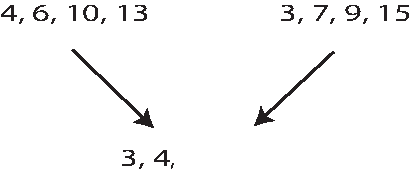
\includegraphics[width=2in]{merge-1.pdf}
}
%\caption{Example binary tree {\tt T} that is passed to {\tt mystery()} function.}
%\label{fig:tree-T}
\end{figure}


3. If you have two lists each of size $N/2$, what is the worst case number of comparisons that will be required to merge the two lists? 

4. Describe your algorithm for merging the two lists.

\newpage

5. The merge phase of the Merge Sort initially merges two adjacent lists of size one into one ordered list of size two. It then merges two adjacent lists of size two  into one list of size four, and so forth. It continues until it merges two lists, each of size $N/2$, into one list of size $N$. Complete the merge phase, beginning  with the following $N$ lists of one number. Continue until you have one ordered list of size $N$.


\begin{figure}[h]
\centerline {
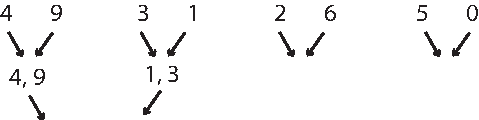
\includegraphics[width=3in]{merge-2.pdf}
}
%\caption{Example binary tree {\tt T} that is passed to {\tt mystery()} function.}
%\label{fig:tree-T}
\end{figure}

\vspace*{1.5in}
6. Apply the merge sort (both the splitting and merge phases) on the following numbers:

\begin{center}$7, 2, 9, 0, 6, 4, 3, 1$\end{center}


\vspace*{2in}

Analyzing the Merge Sort

7. Answering in terms of $N$, how many different levels are required to split $N$ numbers into $N$ lists of size one?

8. At each level, what is the worst case number of comparisons that may have to be performed during the merge phase? (See your answer to Problem \# 3.) 

9. When you multiply the number of levels by the worst case number of comparisons at each level, you arrive at the function that can be used to determine the Big-oh value of this algorithm. What is your Big-oh analysis?



 \end{document}
